In the world of the web 2.0, web applications are a cornerstone of every interaction users have on the web. These applications have very strict performance requirements: a typical web user will expect a page to fully respond to her request within a few hundred milliseconds. High latencies have shown to drive customers away \cite{akamai}, \cite{akamai2}. In addition, web applications suffer from variable load, with spikes occurring during flash crowd events. However, fully loading a web page often requires accessing data stored on a database, often though multiple parameterized queries of varying complexity. In \cite{manjhi2009}, Manjhi et al. mention that the average number of database queries per dynamic HTTP interaction on web applications they benchmarked varies between 1.8 and 9.1. Furthermore, in the world of Big Data, data volumes are increasing rapidly for web applications which makes answering each query increasingly more resource-consuming.

\begin{figure}[h]
\centering
\begin{minipage}{0.45\textwidth}
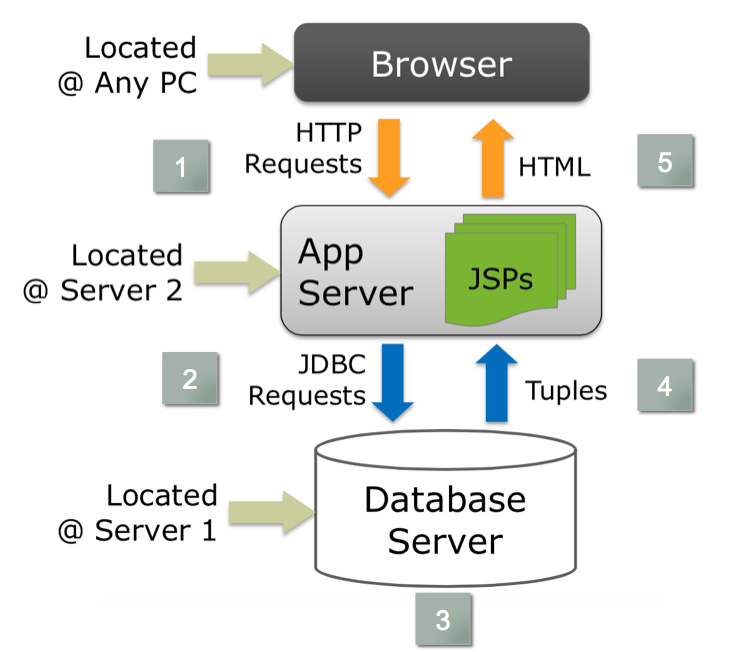
\includegraphics[width=8cm]{images/WebApplicationArchitecture.png}
\caption{Web Application Architecture for Java}
\label{fig:webapp}
\end{minipage} \hfill
\begin{minipage}{0.45\textwidth}
\centering
\begin{Java}[basicstyle=\small]
public List getSumTotals(List selectedNations) {
     List sumTotals = new ArrayList();
     PreparedStatement stmt = conn.prepareStatement(
        "SELECT sum(o.total_price) as sumTotal "
        + "FROM Orders o, Customers c "
        + "WHERE o.cust_ref = c.cust_key "
        + "AND c.nation_ref = ?");
     for (Nation nation : selectedNations) {
         stmt.setInt(1, nation.getNationKey());
         ResultSet rs = stmt.executeQuery();
         rs.next();
         int sum = rs.getInt("sumTotal");
         sumTotals.add(Pair.of(nation, sum));
     }
     return sumTotals;
}
\end{Java}
\caption{Java Code for Example 1}
\label{fig:code1}
\end{minipage} \hfill
\end{figure}


\begin{figure*}[t]
\centering
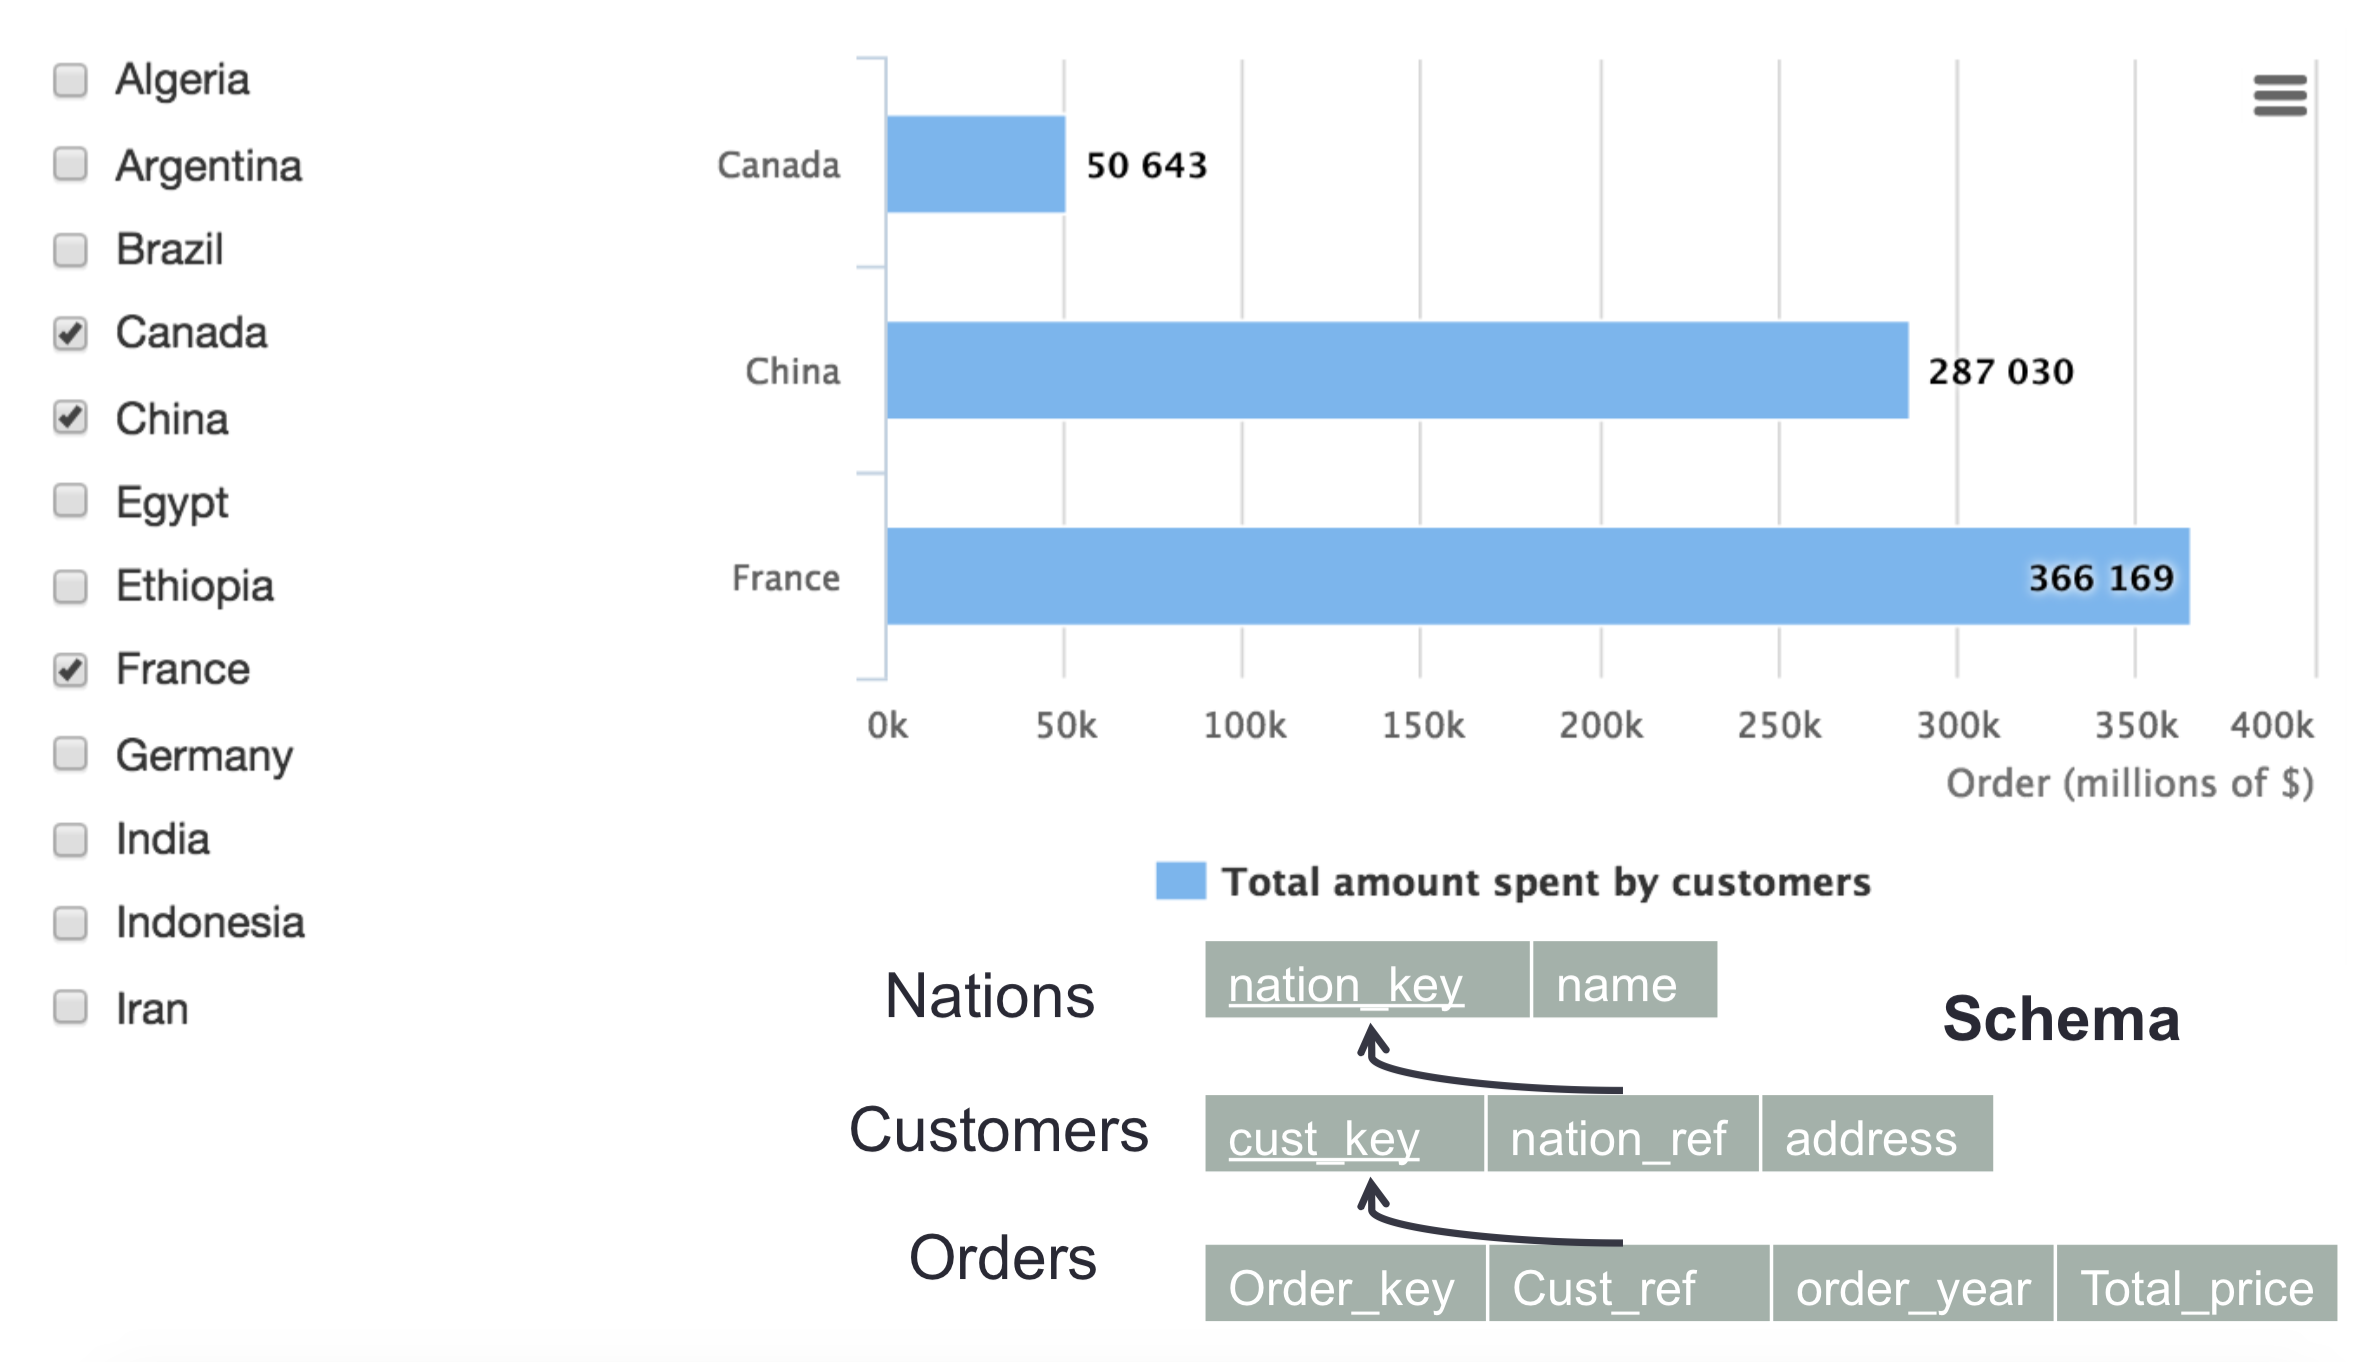
\includegraphics[width=14cm]{images/RunningExample.png}
\caption{Monitor amount spent by customers from selected countries (Example 1)}
\label{fig:example1}
\end{figure*}

To ensure latencies as low as possible, it is important to understand how latency arises. Figure \ref{fig:webapp} describes the architecture of typical web applications and the journey of a user request: \footnote{Note that the architecture on this figure is Java-specific, but the same architecture is used for web application frameworks in other languages such as Python, Ruby or Javascript.} \
\begin{enumerate}
\item{An HTTP request is sent from the browser to the application server, containing the data the user specified when clicking on the web page.}
\item{The request is processed by the application server logic, which in turn sends database queries.}
\item{Each query is compiled, optimized and executed individually.}
\item{The result of the queries are returned to the application program which produces an HTML template with the updated information.}
\item{The HTML result is sent back to the user's browser.}
\end{enumerate}
During this process, latency is dominated by 1) communication over the network in steps 1,2,4,5 (although bandwidth for processing between the application and database servers will typically be higher) and 2) disk I/O to access data from the database.

As a running example, consider the web application shown on Figure \ref{fig:example1}, which describes a dashboard for visualizing and analyzing sales data, based on a TPC-H database \cite{tpch}. A user checks boxes according to the nation she wants to analyze, and the selections are kept as in-memory objects within the HTTP session of the application server. The application then displays an HTML table with the total sales revenue for the selected nations. When the request for new set of checkboxes is issued to the application server, the program on figure \ref{fig:code1} is executed. On line 10, for each \texttt{nation} in the \texttt{selectedNations} list, a parameterized query is issued which computes the desired sum. Each sum computation requires producing a join between two large relations, albeit with a selection on customers based on the nation reference. The results are then accumulated on line 13 and returned for further processing on line 15. We denote this kind of data access pattern a \textbf{parameter-at-a-time} execution.

This execution pattern will iteratively send a SQL query for each requested nation, and each such query will return a single value. This kind of execution comes with two kinds of performance problems : 
\begin{enumerate}
\item{\emph{Network round trip delay}: every SQL query requires a round-trip delay, regardless of the size of the data sent or received. Given that the bandwidth available between an application server and a database server is typically high, and will likely be underused.}
\item{\emph{Repeated disk I/O}:  every SQL query will perform random I/O on the \texttt{Customers} relation followed by a join with the \texttt{Orders} relation, two rather expensive computations.}
\item{\emph{Sequential Execution}: SQL queries are sent to the database sequentially by the application program, which means the latency cost for a single page request will be at least the sum of the costs of each network round trip and disk I/O performed! These queries could, however, be run in parallel.}
\end{enumerate}

Clearly, the parameter-at-a-time execution pattern will be too inefficient if either the data volume or the query load becomes too high. This problem cannot be solved by database compiler alone, because it considers and optimizes each query individually. This problem cannot be solved by the application program compiler either, because the queries are expressed in a language it does not understand (SQL). This problem has been known for decades in the database research community as the impedance mismatch problem \cite{cook:2005aa, maier:1987aa}. The solutions found by researchers over the last decade attempt to solve this problem by \emph{holistic optimization}: making the application compiler aware of database access, giving the query compiler access to more efficient data processing strategies. Notice that while this problem clearly occurs in web applications, it can also occur in non-web applications which make use of a database.

\textbf{Roadmap} Section 2 presents a more efficient data processing strategy, denoted \emph{set-at-a-time} execution, studied by database researchers since the 1980's. Section 3 presents two different approaches to holistic optimization in the research arena which attempt to apply \emph{set-at-time} execution in a database application setting : Query Batching, Query Synthesis. Section 4 presents FORWARD, an all-declarative web application framework developed here at UCSD, which offer a completely different approach in which the application program is also described declaratively; we also compare FORWARD and the other approaches on a number of criteria. Finally in section 5, we propose a future work direction which combines FORWARD and query synthesis to unlock optimization opportunities unavailable before.